\part{Results}

%% This part has the 3 chapters related to the main results. Each chapter has the results from one of the papers prepared.
\chapter{Long-term characteristics of solar resource over the Iberian Peninsula}

\begin{abstract}
%     {\color{red}QUÉ HAY AQUÍ:
%     \begin{itemize}
%     \item El estudio se basa en productividad en lugar de en radiación.
%     \item Overview de la radiación en largo plazo. Relacionarlo con la nubosidad, con los aerosoles. 
%     \item Metodología extrapolable para otros estudios en distintas escalas tanto temporales como espaciales. Y también para otras energías.
%     \item cuestiones difíciles: no se ha calculado cv para los periodos climatologicamente estables. ¿Hay variaciones decadales? Wild indica que el recurso debe estudiarse solo con los 10 años anteriores! ver la complementariedad con esto.
%     \end{itemize}}

  % ** En este capítulo se ha elaborado una meodología que puede aplicarse al análisis de cuestiones energéticas relacionadas con el largo plazo y escalas temporales climatológicas. Por ejemplo: el estudio de la variabilidad interanual o decadal de los recursos de energías renovables, así como de la producción eléctrica con éstas tecnologías. El método utiliza técnicas de clustering, lo que permite la evaluación espacial de estas cuestiones. Además, posibilita indagar en estudios de complementariedad de distintas fuentes, gracias a la simplificación de la estructura espacial aplicando las técnicas de agrupamiento.

  % ** Este capítulo contiene una nueva perspectiva para el análisis cuestiones climatológicas relacionadas con la producción renovable: esto implica una manera alternativa de analizar: tendencias de la radiación, tendencias de la producción, relación con patrones atmosféricos, complementariedad etc.

  % ** Se puede analizar la influencia de distintos patrones sinópticos sobre la producción eléctrica con energías renovablesen el área de estudio.

  % ** Se puede analizar la influencia de los modos de circulación en grandes escalas

  % ** Con este trabajo, se puede estudiar si las distintas conclusiones que se han encontrado en relación con el recurso en el área sur de Europa, o PI se observan de manera diferenciada en los clusters de la Península, de tal manera, que esta clasificación sirva para tomar decisiones de gestión de produción o de implantación de plantas futuras. Además, el cálculo de la produción eléctrica potencial, permite ir más allá en la evaluación de ciertas métricas como la variabilidad, ya que muchos de los efectos observados en el recurso, se ven amplificados cuando se hace el cálculo de producción.

  % *** ¿Puede el análisis de clustering encontrar zonas diferenciadas de variabilidad interanual?
  % *** ¿Puede el análisis de clustering encontrar zonas de complementariedad del recurso solar?
  % *** ¿Se observan en las distintas zonas la influencia de patrones sinópticos para las distintas estaciones?
  % *** ¿Se observan en las distintas zonas la influencia de los modos de circulación atmosférica como la NAO?
  % *** ¿Es extrapolable el método a otras zonas?
  
The spatio-temporal characteristics of different renewable resources like solar radiation, wind and precipitation are very different among them and a detailed understanding of each is important for an adequate planning and management of the electricity system. In this chapter, we elaborate a comprehensive methodology to analyse variability and complementarity of PV production that can be applied for long-term energy questions and for climate scales, but it is not limited to those time-scales or to solar resource thanks to the flexibility of the method.\\

The work is focused on solar irradiation as source of energy for photovoltaic (PV) generation over the Iberian Peninsula, IP, and on photovoltaic productivity, which is defined as the amount of energy generated normalized by the installed capacity at each location.  The IP is an interesting site due to the fact that it is a large area with limitations in the interconnectivity with the rest of the European continent. It is also a complex climatic area [] due to its geographical location and its orograhy, which makes it interesting for testing the methodology.\\%  \textbf{A comprehensive methodology to analyze variability and complementarity of solar resource and PV production among sub-regions of this area is developed.}

% The photovoltaic energy yield is defined as kWh per kW installed, which facilitates the comparison among sub-regions and allows a comparison with other renewable energies like solar thermoelectric or wind energy.

% \textbf{The multi-step approach facilitates the spatial evaluation and comparison among areas and it could be applied to different time resolutions, from a short term analysis to climatological perspective as well as a climate change projections analysis.}
The main steps of the method are the application of an objective clustering algorithm for performing a regionalization of the whole domain, the analysis of the temporal variability of solar radiation and photovoltaic energy yield, and the intercomparison of the obtained clusters for examining their complementarity.\\

\textbf{The approach applied in this chapter means a different perpective to analyse the long-term issues in solar resource as the interannual variability, the influence of the large-scale circulation modes, trends or the synoptic patterns related to its variability. The use of the multi-step scheme allows to simplify the spatial analysis and answer the questions from a more applied point of view.}\\

% Dar los principales resultados en el abstract
  
Data from a satellite dataset of 30 years, which is usually considered as the time for defining a climatology, is used inthis chapter and a long-term overview of solar radiation variability is analyzed over the Iberian Peninsula (IP). The spatial distribution and variability of photovoltaic (PV) power yield is calculated for different tracking systems. The variability is analyzed on an interannual time scale, which is relevant for energy supply security and year-to-year price stability. It shows robustness and stability of solar radiation and PV production on average for the whole domain, but with significant differences among clusters that could allow spatial compensation of PV production. The relationship between the variability of solar irradiation and of PV yield is not uniform among the different clusters. Areas where solar irradiation is higher are more sensitive to tracking type.\\

The whole process described in this chapter provides the information of how solar resource and the PV energy yield perform in a limited area and provide the tools to analyze the relationships between sub-areas and their variability. In this sense, this method can be applied for isolated or nearly isolated electric systems located in regions with a variety of climates, or for interconnected systems involving several countries.\\ 

%{\color{red}PRINCIPALES RESULTADOS DE LA IP}  

\end{abstract}  

%\clearpage
\section{Introduction}

%In the past few decades, there has been an increase in the renewable energies installed capacity. Renewable technology prices have decreased rapidly attracting investors to the sector, and political agreements such as the requirements of the European Commission for 2020 are also driving this trend. For photovoltaic (PV) energy a large growing trend is expected in the next years \citep{eurostat2014chap124}. 
% {\color{red} \begin{itemize}
% \item eliminar todo lo que hay en la introducción que sea general y pueda ir en la intro del principio
% \item añadir información sobre la evolución de la fotovoltaica en españa
% \item añadir en la intro pq españa es interesante climatológicamente
% \item añadir pq se utiliza satélite  
% \end{itemize}}


The natural variability of renewable energy resources like solar radiation and wind presents some challenges for the management of electricity systems, which were designed for conventional technologies like nuclear or thermal power plants. For that reason a thorough knowledge and understanding of space-time features of solar radiation is needed. In the case of solar PV energy,  its variability \citep{Widen2015} can be studied from the perspective of the resource or from the perspective of the PV power output, that includes some aspects of the PV generators involved in variability, like inverters or tilted and tracking panels which increase the complexity of the assessment. There are many studies focused on the short-term variability \citep{Zamo.Mestre.ea2014} that analyzed PV production ramps due to changes in solar incident irradiation associated with cloud motion \citep{Cros2014, IEA-PVPS-T14-1.32015}. Also, the smoothing effect that a well-spread site planning has on the PV production is being investigated \citep{Marcos2012, Perpinan.Marcos.ea2013}.\\

Not only short-term scales are important to address renewable resources intermittency but also longer time scales are relevant in order to make the system more efficient and reliable \citep{Davy2012}. Policymakers, transmission system operators and investment companies, need an accurate evaluation of resources availability in present and future climate conditions for their mid and long-term planning. The analysis of interannual variability has a particular importance in order to assess stability of the resource and the financial viability of renewable energy plants \citep{pryor2006inter}, as well as the likelihood of strong electricity price oscillations like the ones associated for example with the large interannual variations of hydroelectric production.\\

Regarding that perspective of long-term variability of solar resources, there are studies focused on long series from stations \citep{Sanchez-Lorenzo2009, Sanchez-Lorenzo2013, vazquez2012interannual} or reanalysis data that identify low frequency changes in solar radiation, as the “dimming” and “brightening” periods \citep{Wild2005}, that show relationship between solar irradiation and anthropogenic aerosols \citep{Nabat2014a}. Some studies examine the influence of large-scale circulation atmospheric modes like the NAO (North Atlantic Oscillation) on solar radiation \citep{Pozo-Vazquez2004, Jerez2013}, while others study the spatial variability instead of the temporal variability \citep{Gueymard.Wilcox2011a}.\\ 

Some authors make use of regionalization techniques for atmospheric variables in order to analyze them from a climatological point of view \citep{Argueso2011} or for solar energy purposes, mainly for operation and short-term assessment \citep{Zagouras2013, Zagouras2014, Zagouras.Pedro.2014}.\\

In this chapter a multi-step scheme that systematizes the time-space comparison of solar irradiation or photovoltaic productivity among sub-regions of the target area is described, taking into account a large set of factors involved in PV production that could affect the variability of photovoltaic energy yield. Spatial complementarity between clusters is analyzed through correlation coefficients of solar irradiation and PV energy yield time series, showing possibilities for compensating PV production shortages in certain clusters.\\

The analysis over the Iberian Peninsula show that most of the results obtain in previous studies can be also seen with this approach. In addition, the methodology allow to give a clearer spatial answer to the questions as well as to sistematize the procedure.\\

%As an implementation example, we have performed a long-term analysis of interannual variability of PV energy yield over the Iberian Peninsula, IP, which has a special interest as a nearly-isolated electrical system with a high solar energy potential and a variety of different climates. The use of satellite data in the case of study is explained due to the fact that in some regions there are not enough well-distributed ground stations with long records of solar irradiation. For this kind of study, where spatial features are important, gridded data from satellites are a high quality alternative data source.

This chapter is organized as follows: in first place, a description of the methodolgy is presented. Each stage of the multi-step scheme is summarized in section \ref{Methods} and explained in more detail in the Methodology chapter. After that, the clustering algorithm is applied to the irradiation over the Iberian Peninsula and main results are shown.\\

\subsection{Methods}

The whole comprehensive scheme followed is represented in figure \ref{fig:multi_step}, showing the 4 stages and procedures that will be explained in detail in the following section.\\

From data of solar irradiation on the horizontal plane as the starting point of the method, the most common variable obtained from different data sources, the scheme will provide different outputs that can be used to evaluate resource and PV production:\\

\begin{itemize}
\item Regionalization of the area to facilitate the spatial analysis.
\item Resource and energy yield aggregated by areas.
\item Interannual variability of the resource and the PV production.
\item Evaluation of the complementarity of the resource and PV production among areas.
\end{itemize}  
 
\begin{figure}[h!]
\centering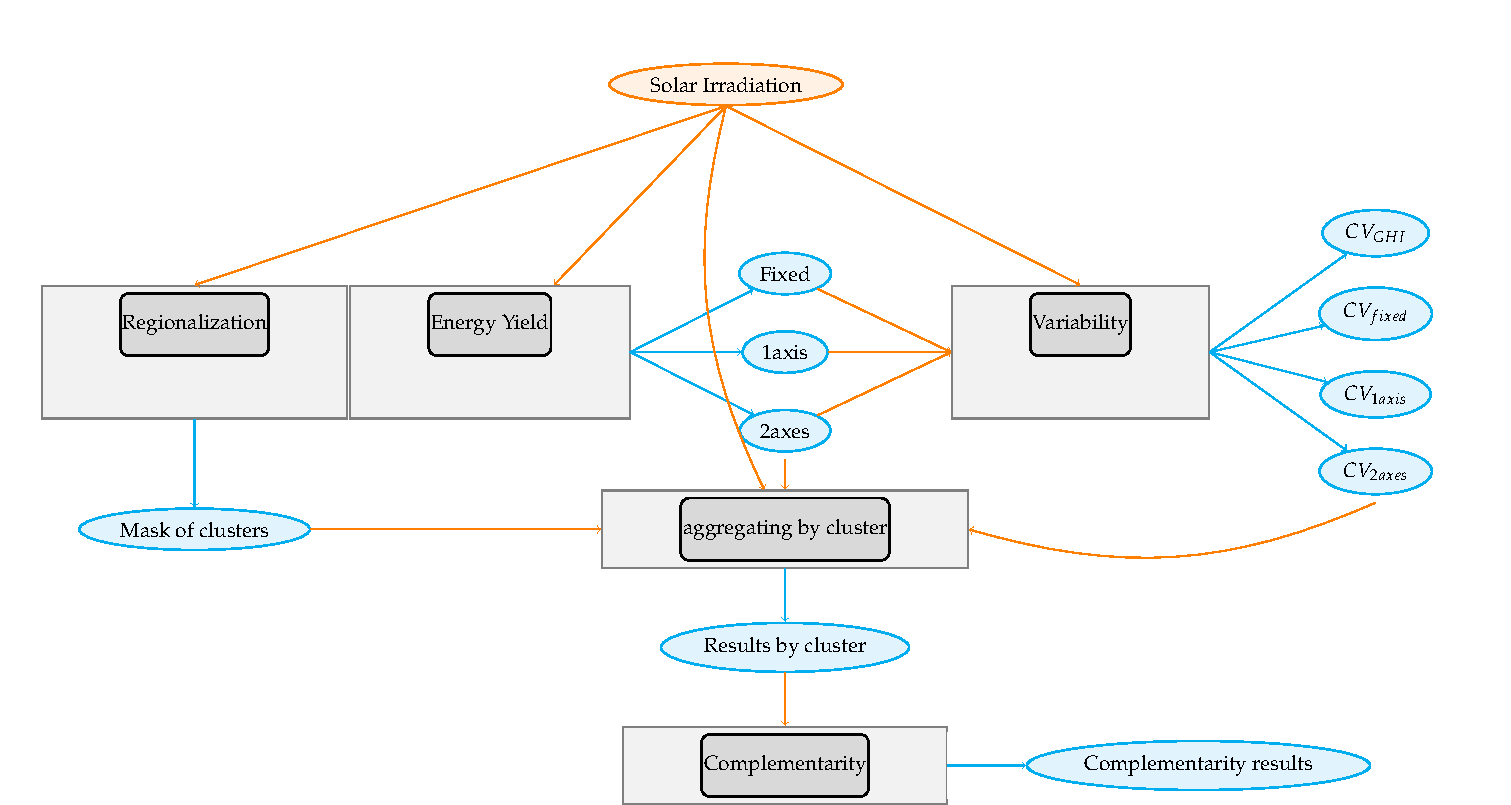
\includegraphics[width=1\textwidth]{figs/capitulo5/multi_step}
\caption{Scheme: Each gray block represents each of the operations needed to get the variability and complementarity results. Orange ellipses are the data employed and blue ellipses are the results of each stage. If the results of one of the blocks are used as input for another stage, connectors are represented in orange color.}
\label{fig:multi_step}
\end{figure}

\subsubsection{Regionalization by clustering}

Regionalization procedures provide the ability of extracting general information of the areas that could be treated as a coherent unit, facilitating the analysis and not considering those characteristics that are not under study. As it was explained in the methodological chapter, classical climatological classifications have some grade of subjectivity due to the fact that they rely on arbitrary assumptions \citep{Kottek2006} and their criteria are based on temperature and precipitation \citep{trewartha1980koppen}. For our purpose, objective and data-derived criteria are more suitable due to the fact that a different variable is analyzed and its classification does not match classical climate divisions. Objective methods based on clustering techniques have been applied successfully over the literature for the analysis of renewable energy resources \citep{Polo2015}, \citep{Zagouras2013}, \citep{Zagouras2014}, \citep{Zagouras.Pedro.2014}, \citep{gomez2015characterization} and atmospheric variables \citep{Argueso2011}, \citep{garcia2012seasonal}. \\

% Clustering methods \citep{Jain1999} can be divided into two categories, partitional and non-partitional. The partitional clustering divides the data into non-overlapping clusters while, the non-partitional or hierarchical clustering, provides a set of nested clusters. In our case, we made use of both algorithms selecting the hierarchical method to initiate a partitional algorithm that is the most suitable for our purpose: to find spatial regions that group together similar time series of the variable analyzed.

A commonly applied regionalization methodology includes the Kmeans algorithm after preprocessing the data through Principal Component Analysis \citep{Ding2004}. This two-step method first reduces redundant information by a Principal Component Analysis that decreases dimensionality of the original dataset. After that, k-means algorithm is applied to the reduced data to find the optimal partition of clusters, which is based on similarity between each element or object inside the cluster and its centroid. This is considered as the most representative element of the cluster, and similarity is measured by an objective function defined in the cluster algorithm.\\

This method presents some problems regarding the random selection of the cluster centroids in the first step. Different initial centroids can lead to different solution or a local optimum could be found. Also, there could be some computational problems if many iterations are needed to get the final partition.\\

The procedure used in \cite{Argueso2011} and in \cite{Zagouras2014} is adapted to get the optimal partition in our scheme from a combined clustering grouping and avoiding the above mentioned problems: the \textbf{k-means partitional algorithm is initialized with a hierarchical clustering solution of a the dimension-reduced data by a Principal Component Analysis.} For the particular case applied in this work, vectors of daily solar irradiation are used for the regionalization. The following steps are needed to get the optimal partition of clusters in the area:\\

\begin{itemize}
\item \textbf{To reduce data dimensionality}. Principal components are eigenvectors of an orthogonal matrix after applied a singular value decomposition (SVD) to the original data, daily solar irradiation vectors, whose initial dimension is reduced to the first eigenvectors that retain $95\%$ of the variance. Considered that, a linear combination of these eigenvectors represents the initial data.
\item \textbf{Hierarchical clustering to initialize k-means}. A hierarchical clustering method classifies data based on a hierarchy. If it is agglomerative, it will start with a cluster for each observation of the data and observations will group together recursively by similarity using the “complete linkage” method. Once the hierarchy is obtained, centroids can be calculated for each emerged partition with a number of clusters between 2 and \textit{n}, where \textit{n} is a high enough selected number of clusters. Centroids will be the initial seed for the Kmeans algorithm, avoiding the computational problems and favoring reproducibility.
\item \textbf{Kmeans algorithm}. The k-means algorithm is a partitional clustering method that minimizes an objective function that defines similarity among the elements of each cluster. In our case we made use of the Euclidean distance, Eq. \ref{eq:euclidean} between the objects or elements in the cluster and its centroid as the objective function. The number of clusters in which the data is divided into has to be known beforehand. In order to overcome the inconvenience, the algorithm is run from 2 to \textit{n} clusters and the optimum number is determined by making use of a clustering validity index after that.
\begin{equation}\label{eq:euclidean}
    J =\sum_{i=1}^{k}\sum_{j=1}^{n}{||x_i-c_j||}^2
\end{equation}


\nomenclature[J]{$J$}{Objective function of the Kmeans clustering method: summation over euclidean distances}
\nomenclature[x_i]{$x_i$}{Each point in the cluster, where the point is a vector with elements comprising the daily irradiation time series values at a pixel obtained from satellite images }
\nomenclature[c_j]{$c_j$}{Centroid of the cluster j}
\nomenclature[PV]{$PV$}{Photovoltaic}
\nomenclature[IP]{$IP$}{Iberian Peninsula}

\item \textbf{Validity index}. In order to determine the optimal partition, validity clustering techniques are applied. There are two types of validation for the clustering methods. First, external clustering validation that make use of external information out of the data; and secondly, there are internal clustering validation methods that rely only on information from the data \citep{5694060}. The latter are used to preserve objectivity as much as possible and are based on two criteria: compactness and separation of the clusters emerged. We use one of the most applied validity index, the Calinski-Harabasz index \citep{CalinskiH}, CH, that evaluates the average between and within cluster sums of squares.
\item \textbf{L-method}. CH index is calculated for every partition from 2 to $n$ clusters. The resulting CH graph in figure \ref{CHindex} for the Iberian Peninsula regionalization is shown for a number of clusters between 2 and 70 as an example. Theoretically, the partition with the maximum CH is the optimum, but the graph shows a decreasing trend which leads to imprecision in finding the optimum. The large number of data and the continuous variable analyzed are responsible for that. For that reason, the L-method is applied \citep{Salvador2004}. This method selects the intersection of two best-fit lines in the graph CH vs. \textit{k}, where \textit{k} is the number of clusters of the partition \citep{Zagouras2013}. All possible pairs of lines that fit linearly to the left and right sequence of data points are created. Each line has at least two points. The total root mean squared error is calculated as in Eq.:\ref{eq:total_RMSE}:

\begin{figure}[h!]
\centering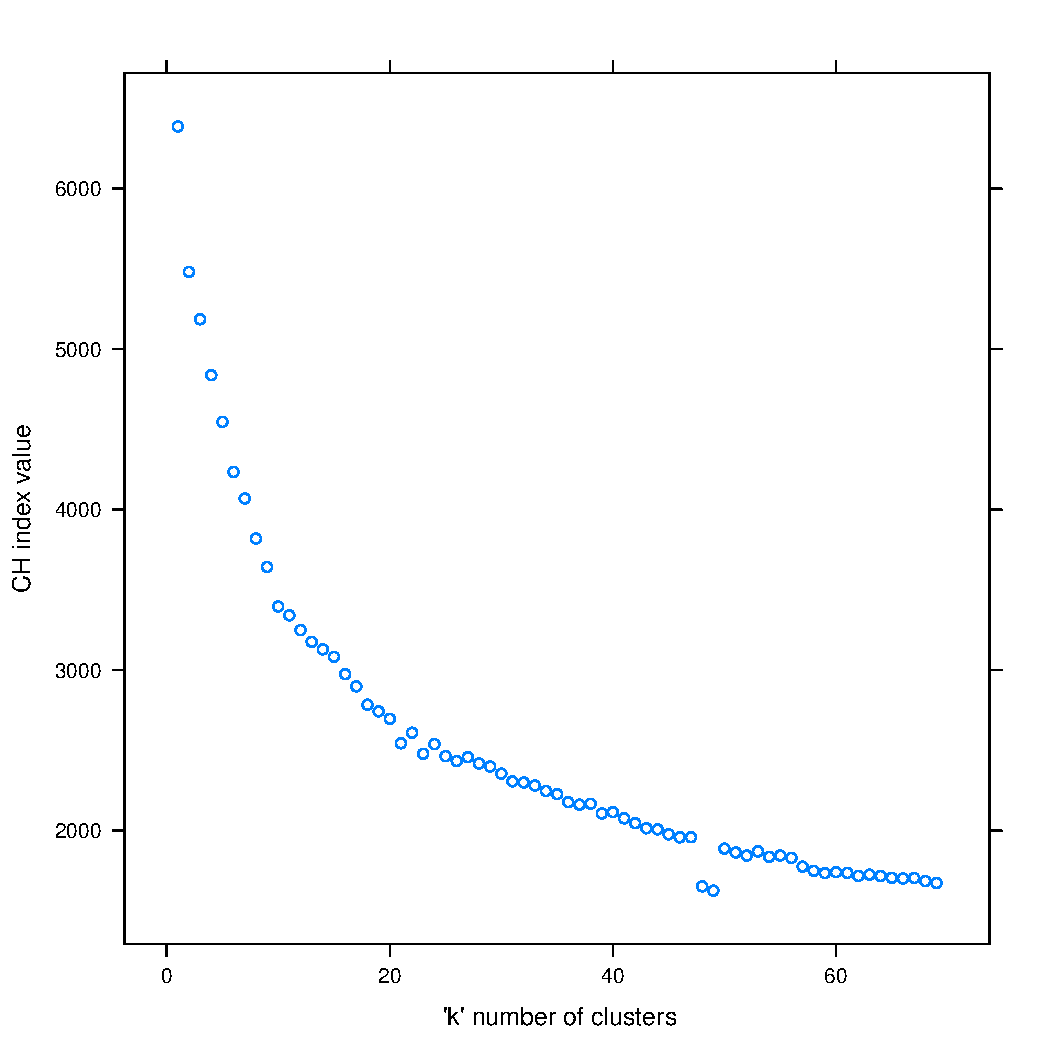
\includegraphics[width=0.5\textwidth]{figs/capitulo5/CHindex}
\caption{Calinski-Harabasz index by 'k' number of clusters}
\label{CHindex}
\end{figure}
 
\begin{equation}\label{eq:total_RMSE}
  RMSE_T = \frac{c-1}{k-1}RMSE_{left}+\frac{k-c}{k-1}RMSE_{right}
\end{equation}


\nomenclature[k]{$k$}{number of clusters.}
\nomenclature[c]{$c$}{number of clusters where the 2 fit-lines split.}
\nomenclature[CH]{$CH$}{Calinski-Harabasz validity index.}
\nomenclature[RMSET]{$RMSE_T$}{Total root mean square error}
\nomenclature[RMSEleft]{$RMSE_{left}$}{Root mean squared error of the left-side linear regression.}
\nomenclature[RMSErigth]{$RMSE_{right}$}{Root mean squared error of the right-side linear regression.}

Where \textit{c} is the number of clusters where the graph is split into the two fit-lines, \textit{k} is the total number of clusters. The ``total root mean square error'' is a weighted error with two terms, one for each side of c in the graph. Each side has a heavier weight depending on the points involved in the fitting. The minimum of $RMSE_{T}$ gives us the optimum number of clusters of the data \citep{Zagouras2013} which are used in the following steps.
 
\end{itemize}
 
\subsubsection{Photovoltaic energy yield}

The simulation of a photovoltaic energy system is described in a previous chapter. Here it is summarized in order to do not miss the coherence of the text.\\

The assessment of the power output of a photovoltaic system is carried out in two main steps:

\begin{enumerate}

\item In first place, global irradiation on the horizontal plane $G(0)$, which is the most common variable obtained from data sources, has to be transformed into the plane-of-array irradiation,  $G(\alpha, \beta)$, where $\alpha$ is the azimuth angle and $\beta$ the inclination angle of the generator plane. Due to optical losses (reflection, angle of incidence, and dust), the irradiation available is reduced for the photovoltaic cells inside the panels and the plane-of-array irradiation is then denoted as effective irradiation on the PV generator $G_{eff}(\alpha, \beta)$.\\
Three different types of tracking types are considered for the photovoltaic generator that influences on the tilt of the panels:
\begin{itemize}
\item \textbf{Fixed} panels with an optimum angle of inclination that depends on the latitude of the place.
\item \textbf{North-South} oriented panels that track the sun daily varying the azimuth angle, we will refer to them as ``one axis''
\item \textbf{Two-axes} tracking system that allows variation of the azimuth and inclination angles, we will refer to them as ``two axes''.
\end{itemize}
  
\item Once the effective irradiation that reach solar cells has been assessed, second step is the transformation into power output that depends on the photovoltaic system. The photovoltaic system is composed of a PV generator, consisting of several PV modules, and an inverter to transform the DC current output from the generator into AC current to be integrated into the network. In order to estimate  potential for photovoltaic production, the term \textit{yield} is defined as the system energy produced divided by the power installed $[\si{\kilo\watthour\per\kilo\wattpeak}]$.

\end{enumerate}

%The detailed description of the transformation from global irradiation in the horizontal plane to global effective irradiation, as well as the methods to assess power output from the PV generator are in the appendix A.

\subsubsection{Variability and complementarity}

The metric to analyze interannual variability is the coefficient of variation, CV Eq.\ref{eq:CV}, which is defined as:

\begin{equation}\label{eq:CV}
  CV=\frac{\sigma}{\overline{X}}
\end{equation}

In this equation, $\sigma$ is the standard deviation of the variable analyzed and it is divided by the mean of the variable in the period of the study. Sometimes CV is represented in percentage. This measure is dimensionless and can be applied in different time scales, which is helpful for comparisons.\\

To assess complementarity of the solar resource in the area of study, the Pearson's correlation coefficient between the time series of pairs of clusters Eq.\ref{eq:pearson} is calculated:

\begin{equation}\label{eq:pearson}
  \rho_{i,j}=\frac{\sigma_{c_i,c_j}}{\sigma_{c_i}\sigma_{c_j}}
\end{equation}

In this equation, $c_i$ and $c_j$ are the time series corresponding to the clusters $i$ and $j$. The concept of complementarity is associated with negative correlations between sub-regions of a wider area. If there is such a complementarity, a positive change in the variable for one of the clusters will be associated to a negative change for the other one. This is relevant for identifying spatial compensation possibilities and reducing overall variability in a network with high penetration of solar PV energy.\\

Complementarity can occur in different scales, either spatial or temporal and to understand it sometimes is a matter of balance. Spatial resolution for the complementarity assessment must be high enough to make sense of the comparison between zones, due to the fact that it is clear that geographically dispersed areas, far from each other, will have very different evolution of atmospheric variables, but may not be interesting from the electricity generation point of view. On the other hand, if the area of study is too small, atmospheric variables and therefore renewable resources will evolve in a very similar way. For such small areas, local complementarity between different resources can be analyzed, but not spatial complementarity of one resource. The methodology presented here addresses this issue by applying the inter-cluster comparison, that ensures homogenity within each cluster and differences between them.\\

Correlation coefficient for a long time series may hide changes in complementarity for shorter sub-periods with higher frquency correlations. For that reason a moving window is applied to the time series calculating the correlation coefficient and providing an indication of how complementarity between clusters varies during the whole period. Width of the window depends on the length of the time-series analysed.\\

In order to obtain the more important cluster pairs regarding complementarity, the median of the correlation coefficient series is calculated for each pair. After that, the cluster pairs are reordered from lower to higher values of this median correlation.\\
%, and the first 15 pairs (with the lowest median correlation) are selected as the most representative of complementarity, altought this number is rather arbitrary and also depend on the length of the time-series analysed.
 

\subsection{Results}

The optimal partition after having applied the clustering method is represented in figure \ref{clusters}. The CH validation procedure gives an optimum number of 19 clusters for the area, where each of the clusters has an homogeneous time evolution of solar irradiation. Due to the nature of clustering techniques, there is not an unique/best method to select the optimum partition. Another index (Davies-Boudin, \cite{davies1979cluster}) has been applied for comparison, and the obtained optimum number of clusters was of the same order than for CH index.
 
\begin{figure}[h!]
\centering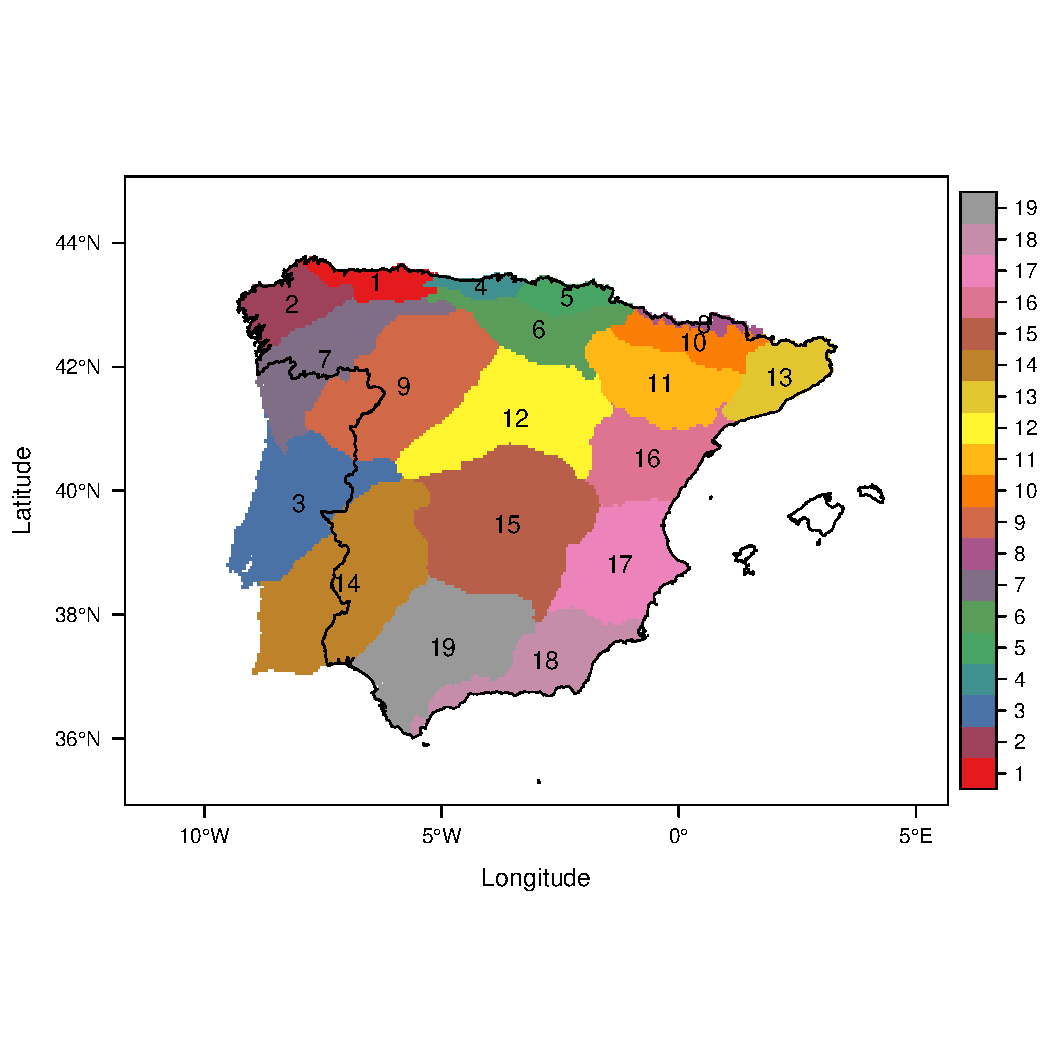
\includegraphics[width=0.6\textwidth]{figs/capitulo5/clusters2}
\caption{Optimal partition of 19 Clusters after applied the algorithm and the validity index}
\label{clusters}
\end{figure}

\subsubsection{Variability and complementarity results}

After regionalization, it is performed an analysis of solar irradiation on the horizontal plane and PV yield by tracking system, including their temporal variability.\\

Regarding interannual variability, we have calculated the CV of two time-aggregated means of solar irradiation and PV yield:

\begin{itemize}
\item On one hand it is applied for the yearly mean of daily irradiation $G_{d,y}(0)$ and yearly PV yield. This metric gives the variation of the of energy from one year to another and if it is low, general stability of the solar resource and PV production is guaranteed. 
\item On the other hand the interannual variability of the monthly time series $G_{d,m}(0)$ and monthly energy yield is also investigated in order to quantify differences in the annual cycle. 
\end{itemize}

The CV is also aggregated by cluster, in order to facilitate the intercomparison among areas.\\

%The general results about yield and variability can be found in the appendix. Here we present particularly relevant results that show the importance of considering different types of tracking methods, which is a fundamental aspect of the proposed scheme.\\

Power from the PV generator depends quasi-linearly with solar irradiation at the plane-of-array ($G_{eff}(\alpha,\beta)$), besides second order effects (spectrum, wind, etc) \citep{Perpinan2007} . Due to that the fixed typology is the one with lower yield because the amount of irradiation reaching cells is lower than the amount of energy reaching panels when trackers have one or two axes movements.

For areas where solar irradiation is higher, yield differences between trackers are higher. This can be seen in figure \ref{yearly_productivity_byCluster} where yearly mean yield for the 30-years period is aggregated by cluster and tracking system, and clusters are sorted vertically from less to more energy yield. A noteworthy result is that yield increase from fixed panels to one-axis panels is non-linear. This increase ranges between $17\%$ for the clusters with less solar irradiation, located at the northern coast (clusters 4, 5), and $30\%$ for the southern clusters with more solar irradiation (clusters 18, 19). In contrast, enegy yield increase from one-axis to two-axes panels is almost constant, around $12\%$ for all clusters. A consequence of the non-linear PV yield increase from fixed to one-axis panels is that the energy yield differences between clusters are much higher for tracking than for fixed systems. While for fixed panels PV energy yield varies between 1000 and 1450 $[\si{\kilo\watthour\over\kilo\wattpeak}]$, for two-axes systems it varies between 1350 and 2100 $[\si{\kilo\watthour\over\kilo\wattpeak}]$. These average values are coherent with results obtained in \cite{Antonanzas-Torres2013} when considering a value of 0.75 for the system performance ratio.
 
\begin{figure}[!tbp] 
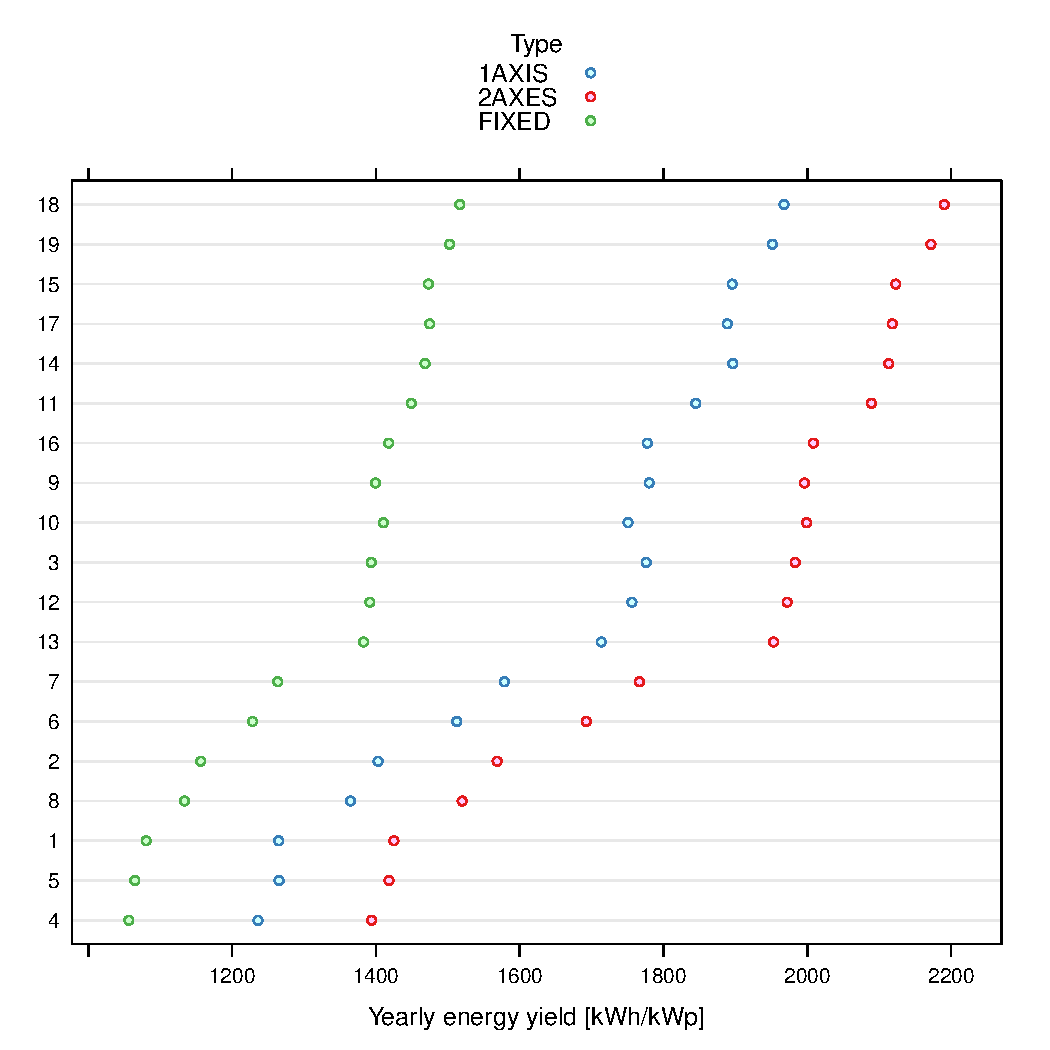
\includegraphics[width=0.6\textwidth]{figs/capitulo5/productividadTemp_byCluster.pdf}
\caption{Yearly mean of PV yield by cluster and for each tracking system $[\si{\kilo\watthour\over\kilo\wattpeak}]$. Values are sort from lower to higher yield values.}
\label{yearly_productivity_byCluster}
\end{figure}

Electricity price variations significantly depend on the variations of the monthly renewable electricity production from year to year. This time-scale is also the most influenced by the large scale circulation modes for solar potential in the Iberian Peninsula \citep{Jerez2013a}. The winter half of the year, from October to March, is especially variable.

The interannual variability for monthly yield is higher than for the irradiation at the horizontal plane, as it occurred for yearly values which results are in the appendix. In winter months, these differences in CV are much higher than in summer. This behavior is more pronounced in northern areas.

In order to quantify these differences in variability between solar irradiation and solar power output, the ratio between variability of yield by tracking system and solar irradiation is represented in figure \ref{ratiosCV} for each month and cluster. If CV of energy yield is higher than CV of solar irradiation, values are above one. On the other side values will be below one if CV of solar irradiation is higher than CV of energy yield. 

\begin{figure}
  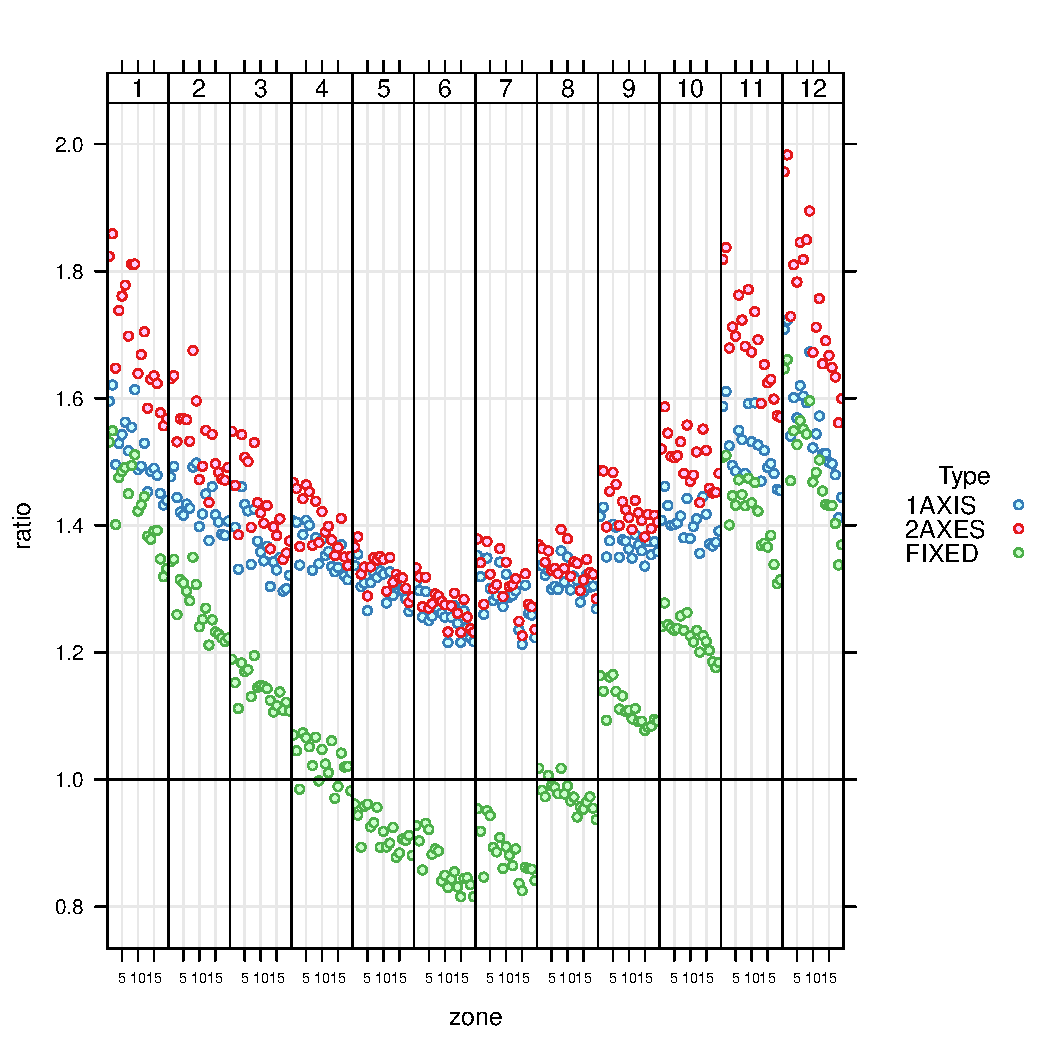
\includegraphics[width=0.6\textwidth]{figs/capitulo5/dotplot_ratio_zone.pdf}
  \caption{CV ratios between each type of tracking system and solar irradiation at the horizontal plane, grouped together by month in the graph. Ratios are calculated for each cluster, represented in the x axis. ``Fixed'' represents $\frac{CV_{fixed}}{CV_{G0}}$, ``1 axis'' is $\frac{CV_{1axis}}{CV_{G0}}$ and ``2 axis'' is $\frac{CV_{2axes}}{CV_{G0}}$}
  \label{ratiosCV}
\end{figure}

The highest ratios are obtained between $CV_{2axes}$ and $CV_{G0}$. The ratio of $CV_{1axis}$ is clearly lower in winter months, but is very similar in summer to the ratio of $CV_{2axes}$. Yield with an 'horizontal' axis tracker and 'two-axes' trackers increase the variability between $20\%$ in summer and more than $80\%$ in some areas in winter. The fixed typology ratio, $CV_{fixed}/CV_{G0}$ has a much wider range in the whole year. In winter months, it has values between 1.2 and 1.6, depending on the cluster, and is not far from the other two typologies. In contrast, this ratio decreases rapidly in summer months, reaching values below one between May and August. This means that for that period, variability of the 'fixed yield' is smaller than variability of solar irradiation at the horizontal plane.

The results of CV show that variability of PV energy yield at tilt panels is higher than variability of solar resource at horizontal plane in most cases, explained by the nature of solar irradiation at tilt panels and its dependency of solar irradiation at horizontal plane, \cite{Perpinan2009}.

The monthly time series are also selected for the complementarity analysis.

Regarding solar power complementarity, opposite-evolving time-series for different areas would strongly increase the reliability of the whole electric system, as shortfalls of solar irradiation in certain areas could be compensated by above-normal irradiation in others. However, this ideal situation is difficult to find in a rather limited area like the IP, at least for monthly timescales over a long time period of 30 years. In this case, the absence of correlation becomes also important, as it avoids simultaneous shortfalls or simultaneous above-normal values, and therefore softens the overall power production. The correlation matrix for the 30-year period and each month is in the appendix, showing the results for the whole period. In most cases, the correlation coefficient is highly positive, specially between pairs in the northern part of the Iberian Peninsula. For the southern part, the correlation coefficient is also positive but it decreases in July and August. There are some exceptions between the northern clusters 4 and 5 and the southern clusters 14 to 19, these pairs are only slightly correlated, not correlated or even slightly anticorrelated for some months.

Overall, southern and eastern clusters are uncorrelated at least during part of the year with northern and northwestern clusters. In some cases, the absence of correlation is found between nearby clusters: in winter months, the north-eastern cluster 11 (central Ebro valley) is uncorrelated to the closely-lying clusters 4, 5 and 8 (in the northern coast and Pyrenees). This is probably related to persistent atmospheric situations with north to northwesterly winds, that cause cloudiness in the windward clusters and clear skies in the leeward Ebro cluster, due to a foehn effect. This result points out the selective character of the clustering method.

It could be that the obtained clusters present higher complementarity in shorter sub-periods. We have divided the whole 30-year period in sub-periods of consecutive 15 years. The correlation coefficients have been calculated again for the resulting 15-year moving window, for each pair of clusters and for each month. In this way, we obtain how each correlation coefficient evolves during the 30 year period. The analysis has been applied for the four variables in the study: solar irradiation at the horizontal plane and PV energy yield for each tracking system.

The median value of the correlation coefficient series is calculated for each pair. Each serie comprises 12 monthly values for each of the 15-year moving windows. After that, the cluster pairs are reordered from lower to higher values of this median correlation, and the first 15 pairs (with the lowest median correlation) are selected as the most representative of complementarity. These cluster pairs are represented in figure\ref{horizonplot_rad}, showing the time-evolution of its correlation coefficient. These results are for solar irradiation on the horizontal plane. The corresponding figures for PV yield by tracking system are not shown due to the similar results obtained for this analysis.

\begin{figure}[h!]
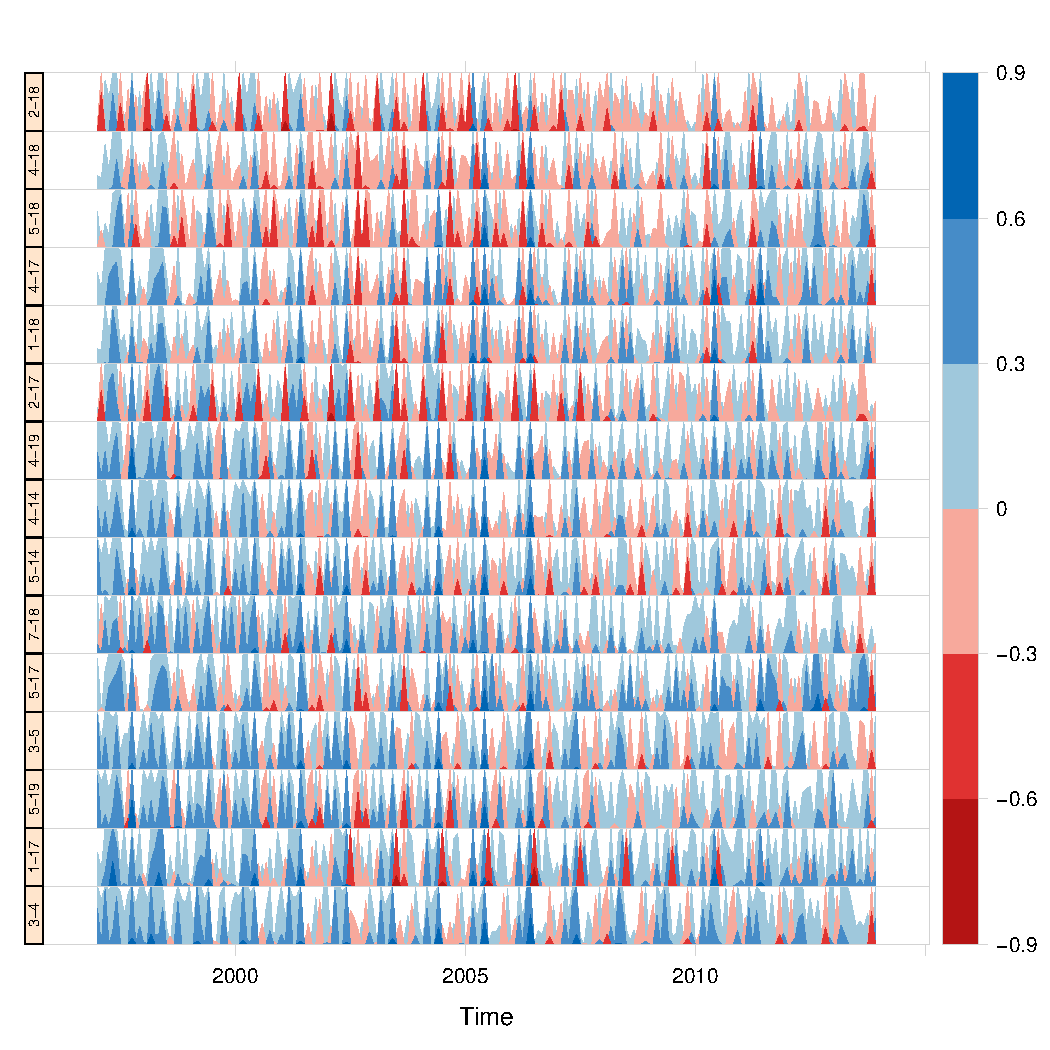
\includegraphics[scale=0.6]{figs/capitulo5/horizonplot_series_rad2}
\caption{Correlation coefficient of solar irradiation at the horizontal plane: evolution of a 15-year moving window of monthly values, for the 15 cluster pairs showing the smallest median correlation values. Monthly negative correlations (in red) and monthly positive correlations (in blue) are represented in the same axis to facilitate the comparison of the multiple time-series. Also, higher correlation values overlap with lower ones, enabling a compact presentation of all the information in a narrower plot. The cluster pairs are indicated on the left, while the year in the x-axis indicates the end of each 15-year moving window.}
\label{horizonplot_rad}
\end{figure}

The most relevant pairs in terms of complementarity include a northern (1, 2, 4 or 5) and a south-eastern cluster (17 or 18), as can be seen in figure \ref{horizonplot_rad}. The negative correlations for these pairs reach values below -0.6, at least in some 15-year sub-periods. These clusters are negatively correlated in most cases. Clusters 19 and 14 (southern and south-western IP) are also negative correlated with clusters in the north, although with lower values than the south-eastern clusters.

It is important to notice the appearance of cluster pairs 3-4 and 3-5 in this figure. These clusters are closer than the previously commented cases, which highlights the adequacy of the clustering method. All three are Atlantic coast clusters, but while cluster 3 includes part of the western coast, clusters 4 and 5 are northern coast areas. This fact, together with the position of the main mountain ranges, can explain their partially complementary behaviour.

%It is important to notice the appearance of cluster pairs 3-4 and 3-5 in this figure. These clusters are closer than the previously commented cases.  All three are Atlantic coast clusters, but while cluster 3 includes part of the western coast, clusters 4 and 5 are northern coast areas. This fact, together with the position of the main mountain ranges, can explain their partially complementary behavior. On the other hand, the 15-year moving window reveals interesting changes with time for all the cluster pairs, as there are higher and more frequent negative correlations in the middle 15-year sub-periods (those ending around 2005). 

In order to highlight the months with maximum anti-correlation,  figure \ref{horizonplot_months_rad} presents, for the same 15 cluster pairs as above, the minimum values of the monthly correlation coefficient (where the minimum for each month is calculated over all 15-year sub-periods). Differences between months are clearly observed in this graph. Only two months (March and June) show consistently positive values of this parameter, and therefore a low complementarity. In the other months, this parameter has predominantly negative values, revealing a certain degree of complementarity. July, August and September show rather low values and relatively high complementarity, which is important as these are months with a high productivity and also include the summer demand peak. In general,  for the second half of the year, the values of this minimum correlation value are lower than for the first half of the year.

\begin{figure}[h!]
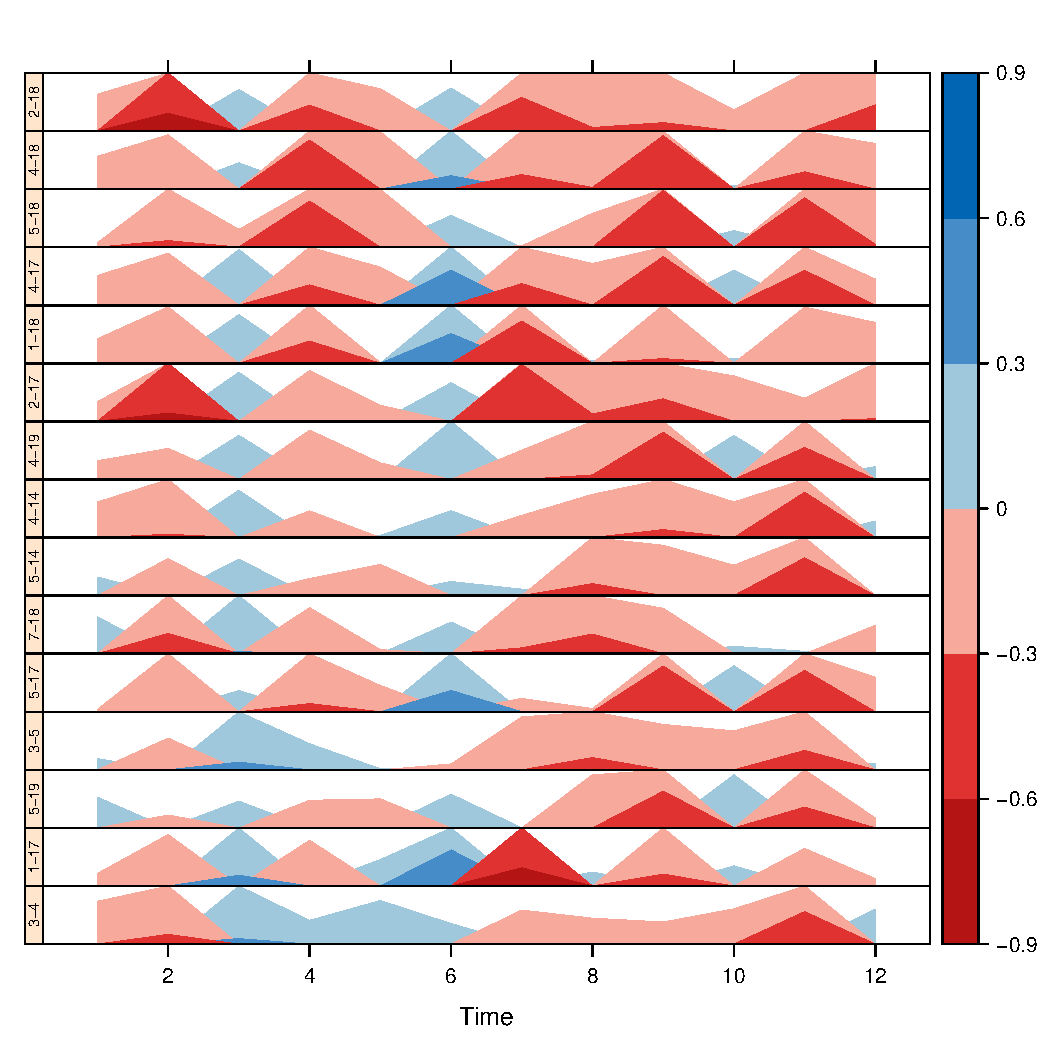
\includegraphics[scale=0.6]{figs/capitulo5/horizonplot_months_rad2}
\caption{Correlation coefficient of solar irradiation at the horizontal plane: minimum values of the monthly correlation coefficient, for the same cluster pairs as figure \ref{horizonplot_rad}. The minimum is calculated over all 15-year sub-periods. The type of representation of correlation values is the same as in figure \ref{horizonplot_rad}. The cluster pairs are indicated on the left, while the numbers in the x-axis indicate the months.}
\label{horizonplot_months_rad}
\end{figure}



\subsection{Conclusion}
\subsection{Summary}

\chapter{Impact of aerosols in photovoltaic energy production over the Euro-Mediterranean area}
\chapter{Future projections of solar resource for photovoltaic applications}

\begin{abstract}

  With the ongoing energy transition, the evolution of renewable energy resources under different climate change scenarios is key for the investors and stakeholders of the energy industry. The possibility of changes in the actual conditions for the operating plants and the projected resources can vary the financial frame of the projects.\\
  
  Although climate models give a robust answer in terms of global warming and other important climate variables, they dissagree in the projected changes of solar resource over Europe. Whereas global climate models, GCM, present a clear positve signal around the mid of XXI century, regional climate models, RCMs show a negative anomaly for the same period.\\
  
  In this chapter we try to explain the reasons behind the different behaviour focusing on the representation of aerosols in the the simulations. We use regional climate models simulations from the EURO-CORDEX project.\\
  
  A fairly pairwise comparison show that regional climate models that include evolving aerosols for the scenarios present the same sign for the signal in the shortwave solar radiation over Europe than global models.\\
  
  We analyse total cloud cover in the regional models simulations and it is not find a clear relationship between the models with aerosols and the anomaly in cloud cover.\\
  
  Due to the clear relationship between sortwave solar radiation anomaly and aerosols evolution, it is necessary to prepare an experiment that is able to give a robust answer in the role of aerosols in terms of shortwave solar radiation projections, which means, that is able to narrow down the uncertainties.\\ 
\end{abstract}

\section{Introduction}

    The generalized increase in the photovoltaic installed capacity in last decades demands the delatiled study of spatio-temporal features of solar resource.\\

  Due to the link between solar energy production and atmospheric variables, there is an increase concern motivated by the availability of resources under climate change scenarios. Due to that, climate modelling is a key tool to evaluate future energy potential despite of some constrains like its low spatial resolution or the coludiness representation.\\
  
   Although variability of solar radiation are mainly due to changes in cloudiness, in clear days other constituents of the atmosphere mostly aerosols, decrease the amount of energy reaching the generator surface. Because of its geographical situation, the Euro-Mediterranean area is one of the most influenced areas by natural and anthropogenic aerosols comming from different sources, affecting the spatio-temporal distribution of solar resource.\\

   Different CMIP5 simulations with different GCMs have been evaluated to assess the photovoltaic potential under climate change conditions (wild et al.) and projecting an increase over Europe. However, later studies using regional climate models (Jerez et al. Bartok) have shown an opposite behaviour, an overall decrease in shortwave solar radiation and photovoltaic potential in the same area.\\

   The added value of regional climate modeling against global simulations lies on the better representation of local features that can not be solved with coarser models. However, the increase in resolution has lead to a simplification of other processes in order to not compromise the computational time. Many regional climate simulations have been done using a very simplistic representation of aerosols content (nabat) and they do not include an evolution of aerosols in future projections.\\
   
   In this work we analyse the evolution of pohotovoltaic potential over Europe for the RCP8.5 scenario usinga regional climate models simulations from EURO-CORDEX initiative. We classify diferent simulations atending to the aerosol representation in the model and its driver global climate model.\\

   Section \ref{Climate data} describes the regional models and simulations used in the study. In section 3 the the main results are explained and a discussion section followed.\\

\section{Climate data: EURO-CORDEX}

\subsection{EURO-CORDEX}

The EURO-CORDEX (Jacob et. al 2014) initiative started as a 'branch' from the Coordinated Regional Climate Downscalling, CORDEX, whose aim is to provide regional climate simulations in different domains. EURO-CORDEX develops climate projections focused on the European continent at different horizontal resolutions (0.44º, 0.11º). These simulations are driven by different CMIP5 GCMs (Taylor et. al 2012).\\

In table 1 there is the information about the aerosols datasets included in the EURO-CORDEX RCMs. It can be observed that only two RCMs from the EURO-CORDEX database include time-evolution of aerosols: RACMO22e and ALADIN5.3. Each of these RCMs have a different dataset of aerosols for projections. Whereas ALADIN5.3 select the Szopa dataset, RACMO22E uses.\\ 

In this work, the choice for the different simulations has followed the next 'pairwise' principle: firstly, RCMs simulations from the EURO-CORDEX database including time evolving scenarios of aerosols are selected. Then, a family of RCMs simulations driven by the same GCMs is constructed around it. Following these steps, we will obtain several groups of RCMs simulations where each one will be called 'family' with the same driven GCM and with only one simulation including aerosols scenarios. Besides, we consider only the RCP8.5 because changes in SSR will be more noticeable and differences between simulations easily detected.\\ 

**La tabla de la descripción de aerosoles de bartok de los GCM se puede referenciar y hacer la de aerosoles de EURO-CORDEX (o de los modelos que yo utilizo?)

\begin{table}
\caption{\label{tb:families}RCMs from EURO-CORDEX and aerosols description grouped by the CMIP5 GCMs drivers.}
\footnotesize
\begin{tabular*}{\textwidth}{@{}lll|lll}
\br
CMIP5 GCM & Institution  & RCM & Aerosols description & evaluation & scenarios\\
\midrule
%  \mr
CNRM-CM5&CNRM&ALADIN5.3&\\
&CLMcom&CCLM4-8-17&Climatology. Tegen 1987\\
&SMHI&RCA4&Climatology\\
\midrule
% \mr  
ICHEC-EC-EARTH&KNMI&RACMO&\\
&CLMcom&CCLM4-8-17&\\
&SMHI&RCA4&\\
\midrule  
HadGEM2-ES&KNMI&RACMO&\\
&CLMcom&CCLM4-8-17&\\
&SMHI&RCA4&\\  
\bottomrule
%  \br
\end{tabular}\\
%$^{a}$UK spelling is required; $^{b}$MSC classification numbers are required; $^{c}$titles of articles are required in journal references; $^{d}$Harvard-style references must be used (see section \ref{except}); $^{e}$final page numbers of articles are required in journal references.
\end{table}
\normalsize

\section{PV potential}

In order to obtain a projection of the photovoltaic productivity over Europe under cliamte change scenarios, a modeling chain approach is considered. Shortwave solar radiation from different climate simulations is used as an input of a photovoltaic model that will give an estimation of the power output. The complete process is explained in chapter 4.\\

The two steps followed in the modeling process of the photovoltaic output are: first, it is necessary to get solar irradiation that reach solar cells, after that the electrical performance of the system is modeled.\\

The process is described in \ref{cha:methods}. In this case, monthly means of daily solar irradiation are used for the decomposition and transformation to the plane of array. Correlation equations between de diffuse fraction and the clearness index described by Page are aplied.   

\section{Results}

\subsection{Anomalies of SSR and CLT}

The anual mean anomaly of the period 2021-2050 for summer months (JJA) with respect to the reference period 1971-2000 is represented in figures 1 and 2 first for shortwave solar irradiation, SSR, and then for total cloud cover, CLT.\\

\begin{figure}[h!]
\centering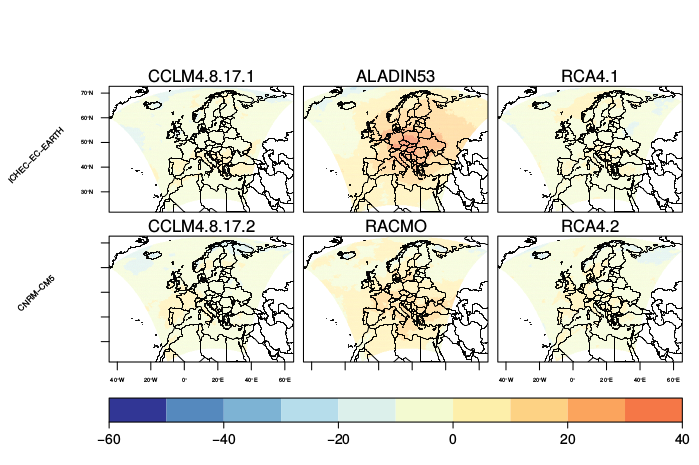
\includegraphics[width=1\textwidth]{figs/capitulo7/ANOMALIAS_JJA_SSR_2050-2021.png}
\caption{}
\label{}
\end{figure}

Anual mean anomaly for summer months shows an increase in Central Europe for climate models with evolving aerosols in scenarios, GCMs and RCMs. In the case of RCMs there are differences in the magnitude of the changes. ALADIN5.3 presents highest anomaly in the mentioned area, which agrees with the anomaly and spatial pattern of aod of this model, as can be seen in figure 3. For RACMO, the aod anomaly has similar spatial pattern but the magnitude is smaller. The same happends with the projected SSR anomalies.\\

The CLT spatial pattern is not complementary with the SSR anomaly map for ALADIN5.3 and RACMO. It means, that the anomaly in SSR is not explained by the anomaly in the total cloud cover. It can be observed, on the contrary that for RCMs with no time-evolving aod the maps are more spatially complementary, as can be also seen in table 3 where values of spatial correlation between both variables are shown. For CM5-ALADIN5.3 and EC-EARTH-RACMO22E the spatial correlation is very low between CLT and SSR and it increase until X and X respectively if AOD is included in the spatial correlation.\\

\begin{figure}[h!]
\centering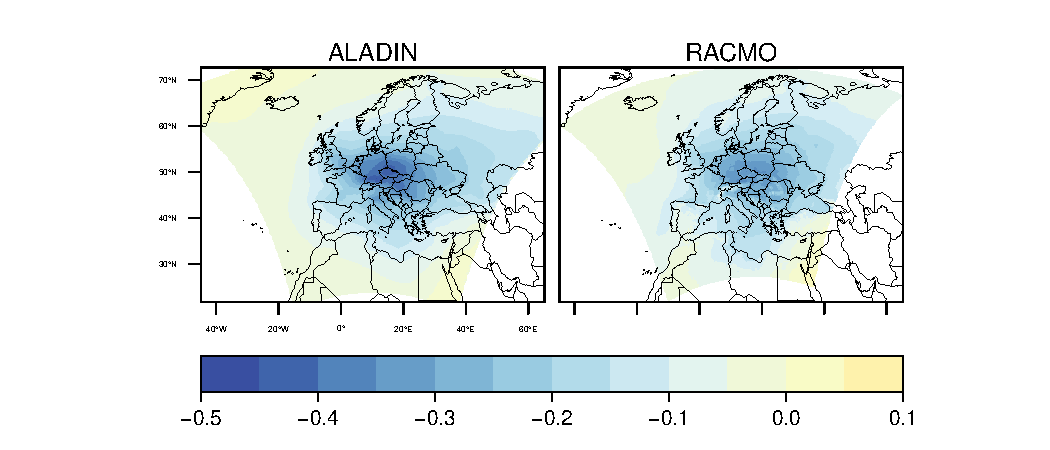
\includegraphics[width=1\textwidth]{figs/capitulo7/ANOMALIAS_JJA_AOD_2050-2021.pdf}
\caption{}
\label{}
\end{figure}

\subsection{Projected changes in PV production}

The photovoltaic yearly productivity, defined as the power output by the power capacity installed (it is consider a 1 kW system for each grid cell), is calculated for each cell of the land in the domain of EURO-CORDEX. Then, the averaged by country of the relative difference with respect to the reference period 1970-2000 is represented in next figure.

{\color{red} Anomalía para los modelos con aerosoles y los modelos sin aerosoles}

The geographical dependence of the PV anomaly is due to the spatial pattern of SSR anomaly, that is close related with the evolution of AOD in central Europe projected by ALADIN5.3 and RACMO22E. It is important to notice that for the simulation including aerosols the sign in PV power output anomaly is positive and negative in the other cases.

Uncertainties due to the different AOD datasets used in the two RCMs and in the radiative transfer code of the model difficults the robust answer about the change magnitude. Averaging the results for the non-aerosols simulations and aerosols simulation, we obtain the results in fugure.

\section{Discussion}

To determine the uncertainity in climate projections is one of the main issues in climate science because the information underlyng the simulations is difficult to comunicate. In order to isolate the uncertainity sources in a multi-model workit is necessary to design a sensitivity test for each of the models in the study. Up to now, there are not enough simulations from the EURO-CORDEX ensemble including evolving aerosols and for those that include them, there is not a the same simulation excluding the aerosols forcing.

For that reason, this preliminary study, although it highlights very important issues is the firs step in order to understand the role of aerosols in the RCM projections.

\section{Conclusion}

% \end{document}